\section{A Quantitative Metric and Our Key Hypothesis}
\label{sec.metric}
In this section, we introduce our metric to quantitatively evaluate security of a kernel. 
%It addresses a gap in that there is no standard method for properly evaluating 
%a system's security level. Thus, 
Our key hypothesis is that \textbf{\textit{commonly used kernel paths}} (or 
\textbf{\textit{common paths}}) contain fewer bugs than \textbf{\textit{uncommon paths}}. 
Our metric provides a fair comparison of different security tools and their impact to the kernel, 
and reveals the portions of the kernel are safe and contain fewer bugs. 

Our experimental results show that only $2.5\%$ of historical kernel bugs that we examined are 
found in common kernel paths, whereas $50\%$ of the bugs are found in the total 
reachable kernel paths. This measurement suggests a new design that 
places limited trust in the entire kernel space (\S{\ref{sec.design}}). 
We then build a prototype Lind, as an example implement of this new design 
(\S{\ref{sec.implementation}}). 

%%%% this subsection repeats the previous sections %%%%%%%
%\subsection{Rationale Behind Our Metric}
%As discussed previously (\S{2}), %a key reason that existing techniques 
%%fail to provide strong protection to the kernel is that there has yet to be a good way 
%%or standard method to understand which portions of the kernel are safe 
%%and which portions of the kernel are risky. 
%we need to gain more knowledge about how the kernel should be exposed to user applications, 
%and how to protect the interactions between the kernel space and 
%the user space without drastic changes to the current kernel structure. 
%Therefore, a metric to help understand this problem is desirable. 
%%and could have huge practical impact. 
%%
%%In addition to having a standard method for measuring and evaluating the kernel, 
%Additionally, such a metric would be a solid basis for comparison between different tools that try to 
%provide secure environment for running programs. 
%Currently, researchers and developers did not have a good way to evaluate the security features 
%of their tools. 
%%let along conduct comparison between different tools. However, to achieve the 
%%goal of building and deploying secure systems, it would be very helpful if we could conduct fair and accurate 
%%comparison between different tools. 
%Our metric provides a quantitative way to 
%facilitate such comparison. An example of comparison of evaluating security features among different tools is 
%demonstrated in our evaluation (\S{6}).

\subsection{Analyzing Kernel Traces}

{\bf Key hypothesis: commonly used kernel paths contain fewer bugs.}
%Now, to address the problem that motivated our metric from the very beginning, which portions of the kernel 
%are safe and which portions of the kernel are risky. We can use our metric to answer this question. To be more
%specific, 
Our hypothesis is that commonly used kernel paths are likely to be safe and contain fewer bugs 
than uncommonly used kernel paths. 
Here, ``commonly used kernel paths'' refer to the kernel paths executed by popular 
applications, such as Web browsers, file editors, etc. 
Our reason is that commonly used kernel paths are used
frequently and therefore bugs and vulnerabilities would have most likely
been caught by developers.  In addition, commonly used kernel paths usually 
include kernel functions that are used in normal ways rather than special 
corner cases. This means that the chances 
to harbor kernel bugs in those commonly used kernel paths are slim. 

%As discussed previously (\S{\ref{sec.motivation}}), we need to gain more knowledge 
%about how the kernel should be exposed to user applications. 
Since we hypothesize that 
common kernel paths contain fewer bugs than uncommon paths, we want to 
evaluate the security a kernel. We achieve our goal with two key steps. First, we capture the 
\textbf{\textit{kernel trace}} of which lines of code in the kernel get executed when running 
popular applications. Second, this kernel trace is checked against the historical kernel 
bugs to see if it contains kernel vulnerabilities. If common kernel paths contain 
fewer bugs than uncommon paths, our hypothesis is then verified. 

{\bf Capturing kernel traces.}
The first step is to capture the lines of kernel code get executed when 
running applicaitons. The OS kernel code is organized under different kernel directories. 
Whenever an application tries to access system resources, such as I/O, memory, and CPU, the kernel code 
under corresponding paths is executed. Therefore, the kernel code execution 
%can be viewed as the fundamental activities of the kernel, and it 
reflects the basic behavior of the kernel, in response to user application requests. 
Thus, %it makes sense to measure and analyze which lines of code get executed in the kernel. 
our metric %adopts this fundamental approach. It 
first captures which lines of code in the kernel get executed 
when running a task program (a user application). We call the 
resulting captured lines of code a \textit{kernel trace}. A kernel trace is closely
related to the task program that generated the trace. Therefore, 
by using the kernel traces, a comparison between different security tools 
%\yanyan{"tools and environments" is confusing. Do you mean 
%applications? security tools?} 
%\yiwen{I mean security tools, such as VirtualBox, Graphene, and Lind} 
is possible. To capture the kernel trace, 
we use \texttt{gcov}~\cite{gcov}, a program profiling tool that is part of the Linux kernel.
%\yanyan{Is it part of Linux kernel? It is "a standard utility with the GNU Compiler Collection (GCC) suite"
%according to wikipedia http://en.wikipedia.org/wiki/Gcov} 
%\yiwen{Yes, it is. We may need to explain a bit more about Gcov and how to use it. 
%But it is just a tool we used, not a key part of the paper.}

{\bf Evaluating the security of kernel traces.}
The second step is to evaluate security aspects of the kernel traces that we captured. Using the historical kernel vulnerability 
reports, we collect a list of severe kernel bugs from the National Vulnerability Database \cite{NVD}. 
For each bug, we identify the lines of code 
in the kernel that would trigger the bug. 
This is done by examining the patch of the Linux kernel source code to fix the bug. 
From the patch, we can identify which lines of kernel code need to be modified in order to remove 
the bug. We thus have the information about which lines of kernel code would trigger the bug. 
We determine that the lines of code in the kernel are \textit{risky} if they 
may trigger one or more kernel vulnerabilities, and those lines of code that cannot trigger kernel vulnerabilities are 
considered to be \textit{safe}. This provides us in-depth knowledge about the safety of 
different portions of the kernel.
%portions of the kernel are risky. 

%In this section, we use our metric to get an idea of which lines of code in the kernel contain fewer bugs, and 
Using the above kernel trace analysis, we empirically label the lines of code in kernel that contain fewer bugs
as \textit{safe lines}. The safe lines of code would then compose the safe portions of the kernel, which can 
be trusted to build a secure trusted computing base for secure systems (\S{\ref{sec.design}}). 
\yanyan{seems kernel coverage is not accurate as the name of the metric?}

%\cappos{I feel it is a bit too much future tense here.  We did verify it.
%It is fine to say we have a hypothesis, and that we provide some initial
%results to confirm it.}
%%If our hypothesis can be verified, then it would become a critical guideline to create new designs for secure systems 
%%(shown in \S{4}). 
%%But before going too far into the new designs, let us first verify that our hypothesis indeed holds, that 
%%commonly used kernel paths are likely to contain fewer bugs and be safe. 
%\yanyan{I feel this paragraph can be cut.}
%\yiwen{We might lose this paragraph.}
%We verified our hypothesis in the following section \S{3.4}. This finding helps form critical guideline to 
%create new designs for secure systems (shown in \S{4}). 

\subsection{Verification of Hypothesis}
%So to verify our hypothesis that commonly used kernel paths contain fewer bugs, we 
%first needed to obtain the commonly used kernel paths. 
%We generated the commonly used kernel paths by using and combining two approaches, 
%system call fuzzing and running popular user applications.  \cappos{I'm
%confused about how fuzzing fits in here.}

To verify our hypothesis that commonly used kernel paths contain fewer bugs, we first 
obtain the commonly used kernel paths, and the total reachable kernel paths. The common paths 
is a subset of the total reachable kernel paths. We show that only 2.5\% of the bugs we examined were 
found in the common paths, while 50\% of the bugs were found in the total reachable kernel paths. 
Our results confirm that common paths contain fewer bugs than uncommon paths.

We obtain the common paths and the total reachable paths as follows. 
%The common paths were captured by running popular user applications, while the total reachable paths 
%were captured by doing system call fuzzing and running Linux kernel test suite. 

%User space applications interact with the kernel space essentially through the system call API. 
%So all those system calls are at the bottom level, while the applications sit at the top level. 
%It makes sense then to obtain the kernel trace from both of those two different levels. 
%We used two different approaches to obtain the kernel trace of commonly used kernel paths. 
%Experiments of both approaches were conducted using the native Linux environment.

\textbf{1) Common paths} are captured by running popular user applications.
We ran applications that are commonly used by many users on a daily basis, such as a Web browser, 
file editor, and so on.  

\textbf{2) Total reachable paths} are captured by system call fuzzing and running Linux kernel test suite. 
We tried to capture the total reachable paths in the kernel as complete as possible. 
Two approaches were combined to capture the reachable kernel trace. 
\yanyan{add one sentence to explain why we need two combined, and why one is not enough.}

First, our system call fuzzing used Trinity system call fuzz tester~\cite{Trinity}, 
and ran system calls exhaustively with all possible 
arguments and options. We fuzzed over more than 300 available system calls, including
file management system calls and network system calls, which gave us a thorough kernel trace. 
In addition, we ran a Linux kernel test suite, Linux Test Project (LTP) \cite{LTP} 
to help capture the total reachable kernel trace. 
Linux Test Project is a mature and well maintained tool to test the Linux kernel. We ran all the available system call 
test cases with this tool to capture the kernel trace. 
Combining the kernel traces generated by Trinity and LTP, we got our reachable kernel paths.


\begin{table}%[ht]
\centering
\scriptsize
\begin{tabular}{|l|c|}
  \hline
  \textbf{Kernel Paths} & \textbf{Kernel Coverage (percentage)} \\
  \hline \hline
  Common Paths & 12.4\% \\
  \hline
  Total Reachable Paths & 32.2\% \\
  \hline
\end{tabular}
\caption {Kernel Coverage}
\label{table:kernel_coverage}
\end{table}

\subsubsection{Coverage Analysis of Common Paths}
The kernel trace coverage of the common paths and the total reachable paths are shown in Table~\ref{table:kernel_coverage}. 
A further breakdown of the composition of the kernel trace is illustrated in Figure~\ref{fig:subset} and Figure~\ref{fig:key_paths_trace}.
%
The results from Table~\ref{table:kernel_coverage} show that the size of commonly used kernel 
paths is small: merely $12.4\%$ of the entire kernel code base. The common paths coverage
is also significantly smaller than the total reachable paths coverage (about $1/3$ of the entire kernel). 
%This shows that commonly used kernel paths are likely to contain 
%few bugs, since the coverage of the commonly used kernel paths is small and leaves little space for vulnerabilities to exist. 
%\yanyan{The small portion does not directly relate to contain few bugs.}
The results from Figure~\ref{fig:subset} and Figure~\ref{fig:key_paths_trace} show that the common paths are a subset of the total reachable paths, shown by the ``OverlappedPaths'' in Figure~\ref{fig:subset} and ``OverlappedLines'' in Figure~\ref{fig:key_paths_trace}. \yanyan{Add 1 or 2 sentences to analyze the figures.}

\begin{figure}%[h]
\centering
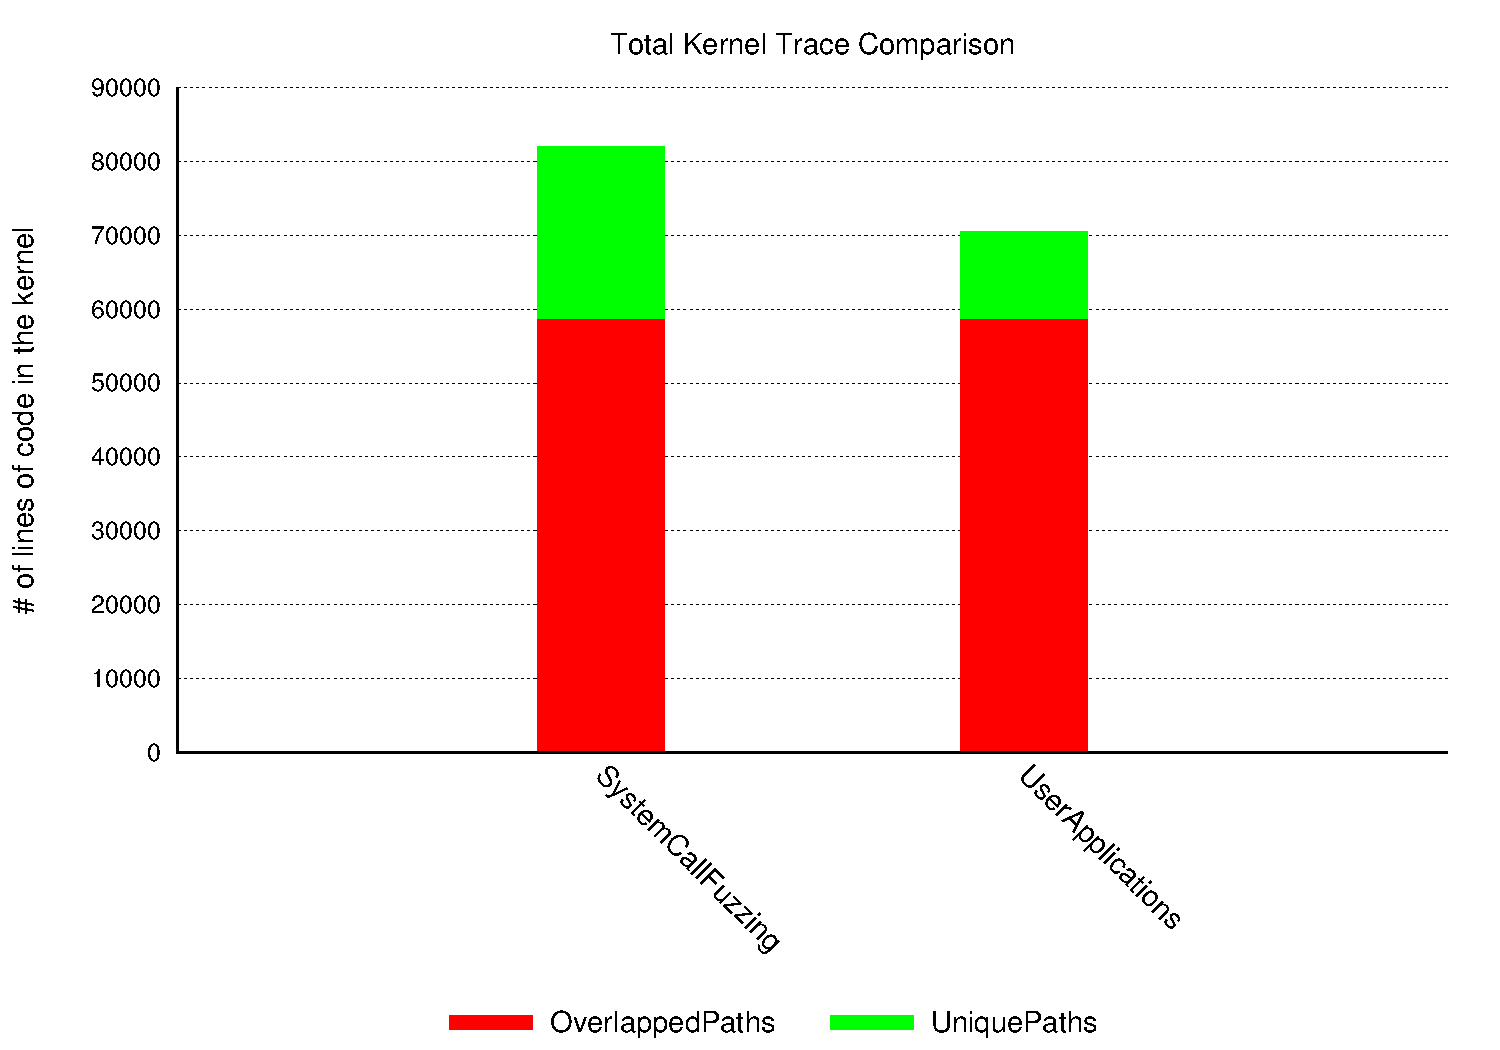
\includegraphics[width=1.0\columnwidth]{diagram/lind_ccs15_diagram_01.pdf}
\caption{Kernel Trace Comparison: Common Paths are Subset of Reachable Paths \yanyan{may put \% numbers beside two bars, 
also remove the caption in the figure.}}
\label{fig:subset}
\end{figure}

\begin{figure}%[h]
\centering
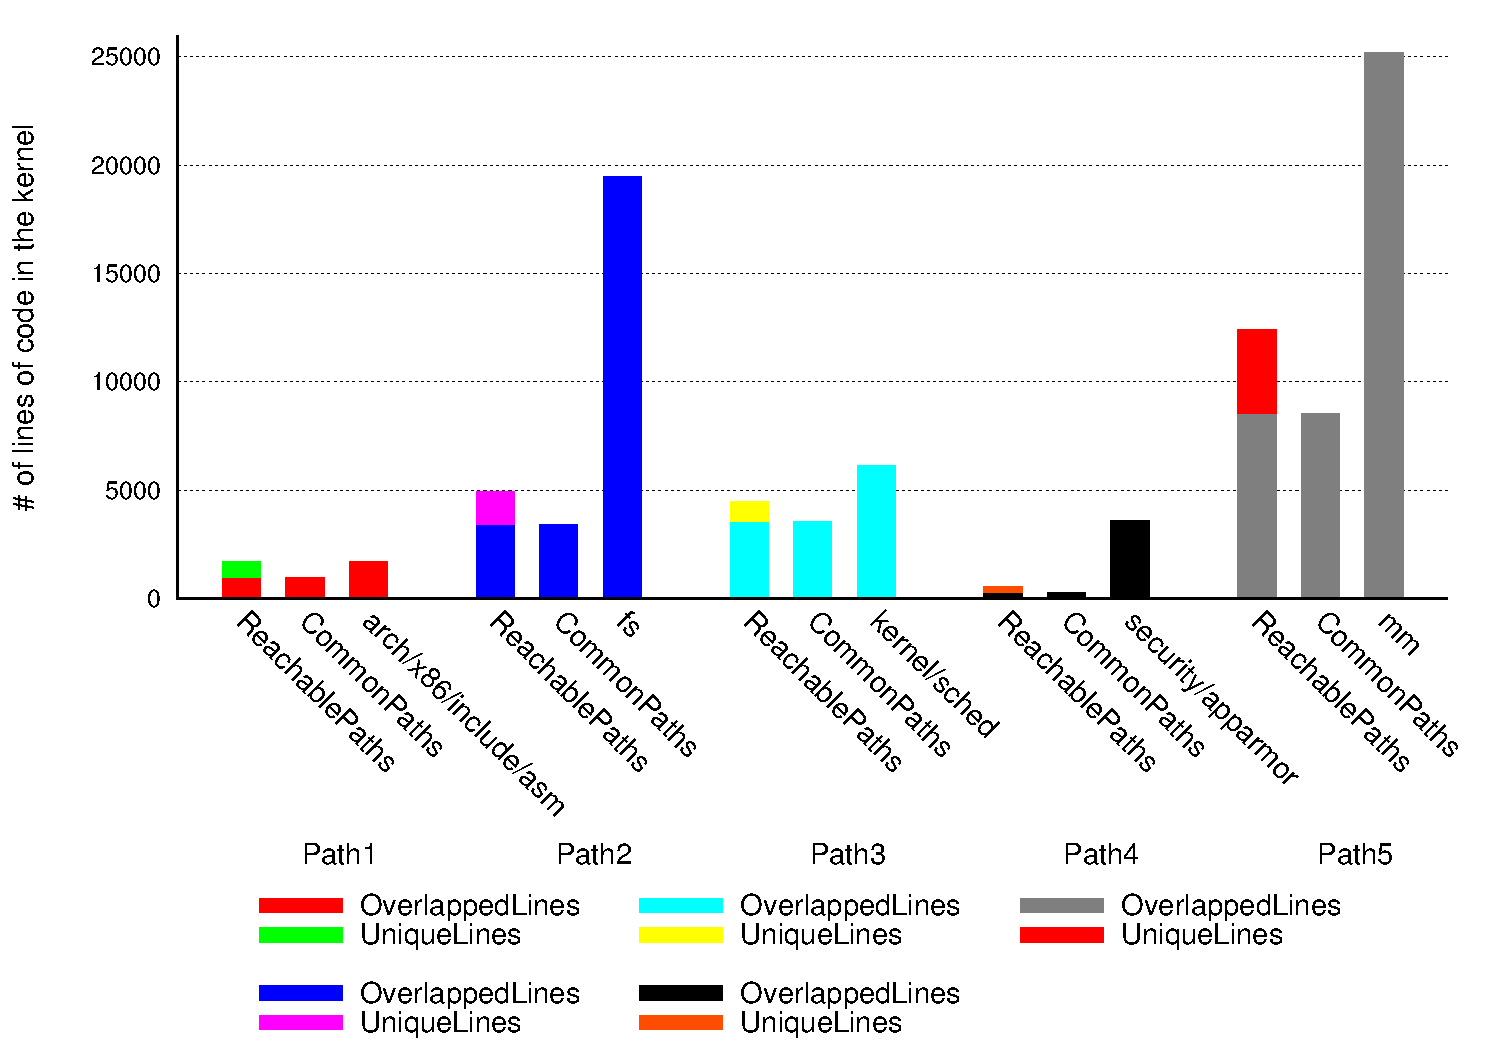
\includegraphics[width=1.0\columnwidth]{diagram/lind_ccs15_diagram_02.pdf}
\caption{Kernel Trace in Key Paths}
\label{fig:key_paths_trace}
\end{figure}


\subsubsection{Security Analysis of Common Paths}
We then checked which portions of the kernel contain more/fewer kernel bugs. 
We examined 40 severe Linux kernel bugs from the last five years (the first two columns in Table~\ref{table:vulnerabilities_commonly_used_kernel_paths}). 
We used these kernel bugs to check if there exist vulnerabilities in certain kernel traces.
The results of our experiment are shown the last two columns in Table~\ref{table:vulnerabilities_commonly_used_kernel_paths}.  
%\cappos{I'm confused.  Does this mean that almost all bugs couldn't be
%triggered with the fuzzing tools?  If so, then the tools themselves seem
%like they are terrible or else we are doing something wrong.  Is there a
%better way to get code coverage / test coverage in the kernel?  Do they
%have tests we can use for this?}
%\yiwen{fixed. please see new results.}

%\begin{table}[!ht]
%\scriptsize
%\begin{tabular}{|l|l|}
%\hline
%%\multicolumn{2}{|c|}{\bf Linux Kernel Bugs Examined} \\\hline
%\textbf{Vulnerability}    &  \textbf{Specific Type} \\\hline
%
% CVE-2014-9529 \cite{CVE:20149529} & concurrency, race condition \\
% CVE-2014-3631 \cite{CVE:20143631} & NULL pointer dereference \\
% CVE-2012-6657 \cite{CVE:20126657} & network socket variable mischeck \\
% CVE-2014-5207 \cite{CVE:20145207} & privilege escalation \\
% CVE-2014-5206 \cite{CVE:20145206} & privilege escalation \\
% CVE-2014-3153 \cite{CVE:20143153} & privilege escalation \\
% CVE-2014-2851 \cite{CVE:20142851} & privilege escalation \\
% CVE-2014-2706 \cite{CVE:20142706} & race condition, DoS \\
% CVE-2014-0100 \cite{CVE:20140100} & race condition, DoS \\
% CVE-2014-0049 \cite{CVE:20140049} & buffer overflow \\
% CVE-2012-6638 \cite{CVE:20126638} & DoS \\
% CVE-2014-0038 \cite{CVE:20140038} & privilege escalation \\
% CVE-2013-6368 \cite{CVE:20136368} & privilege escalation  \\
% CVE-2013-4587 \cite{CVE:20134587} & index error, privilege escalation \\
% CVE-2013-4563 \cite{CVE:20134563} & size/boundary check, DoS \\
% CVE-2013-4348 \cite{CVE:20134348} & value validation error \\
% CVE-2013-4300 \cite{CVE:20134300} & privilege escalation  \\
% CVE-2013-1943 \cite{CVE:20131943} & privilege escalation \\
% CVE-2013-2094 \cite{CVE:20132094} & privilege escalation  \\
% CVE-2013-3301 \cite{CVE:20133301} & NULL pointer dereference, DoS \\
% CVE-2013-1858 \cite{CVE:20131858} & privilege escalation \\
% CVE-2013-1797 \cite{CVE:20131797} & use-after-free \\
% CVE-2013-1763 \cite{CVE:20131763} & privilege escalation, index error \\
% CVE-2013-0310 \cite{CVE:20130310} & NULL pointer dereference \\
% CVE-2012-2136 \cite{CVE:20122136} & heap-based buffer overflow \\
% CVE-2012-2100 \cite{CVE:20122100} & lack of sanity check \\
% CVE-2012-0028 \cite{CVE:20120028} & privilege escalation \\
% CVE-2011-2517 \cite{CVE:20112517} & privilege escalation, buffer overflow \\
% CVE-2012-2123 \cite{CVE:20122123} & privilege escalation \\
% CVE-2012-1146 \cite{CVE:20121146} & NULL pointer dereference \\
% CVE-2012-0207 \cite{CVE:20120207} & divide-by-zero error and panic \\
% CVE-2011-2525 \cite{CVE:20112525} & NULL pointer dereference \\
% CVE-2011-1076 \cite{CVE:20111076} & NULL pointer dereference \\
% CVE-2011-2184 \cite{CVE:20112184} & NULL pointer dereference, none initialization\\
% CVE-2010-2478 \cite{CVE:20102478} & integer overflow \\
% CVE-2010-2960 \cite{CVE:20102960} & NULL pointer dereference  \\
% CVE-2010-2492 \cite{CVE:20102492} & privilege escalation, buffer overflow \\
% CVE-2010-2240 \cite{CVE:20102240} & stack overflow \\
% CVE-2010-1188 \cite{CVE:20101188} & use-after-free \\
% CVE-2010-0437 \cite{CVE:20100437} & NULL pointer dereference \\
%\hline
%\end{tabular}
%\caption {Linux Kernel Bugs Examined}
%\label{table:kernel_bugs}
%\end{table}

\begin{table*}[!ht]
\scriptsize
\centering
\begin{tabular}{|l|l|c|c|}\hline
%\multicolumn{3}{c}{Vulnerabilities in Commonly Used Kernel Paths} \\\hline
\multirow{2}{*}{\textbf{Vulnerability}} & \multirow{2}{*}{\textbf{Specific Type}} & \multicolumn{2}{c|}{\bf Portion of the Kernel} \\
\cline{3-4}
&  & \textbf{Total Reachable Paths} &  \textbf{Common Paths} \\ \hline

 CVE-2014-9529 \cite{CVE:20149529} & concurrency, race condition & {\color{red}\ding{51}} & \ding{55} \\
 CVE-2014-3631 \cite{CVE:20143631} & NULL pointer dereference & {\color{red}\ding{51}} & \ding{55} \\
 CVE-2012-6657 \cite{CVE:20126657} & network socket variable mischeck & {\color{red}\ding{51}} & \ding{55} \\
 CVE-2014-5207 \cite{CVE:20145207} & privilege escalation & \ding{55} & \ding{55} \\
 CVE-2014-5206 \cite{CVE:20145206} & privilege escalation & \ding{55} & \ding{55} \\
 CVE-2014-3153 \cite{CVE:20143153} & privilege escalation & \ding{55} & \ding{55} \\
 CVE-2014-2851 \cite{CVE:20142851} & privilege escalation & \ding{55} & \ding{55} \\
 CVE-2014-2706 \cite{CVE:20142706} & race condition, DoS & {\color{red}\ding{51}} & \ding{55} \\
 CVE-2014-0100 \cite{CVE:20140100} & race condition, DoS & {\color{red}\ding{51}} & \ding{55} \\
 CVE-2014-0049 \cite{CVE:20140049} & buffer overflow & \ding{55} & \ding{55} \\
 CVE-2012-6638 \cite{CVE:20126638} & DoS & {\color{red}\ding{51}} & \ding{55} \\
 CVE-2014-0038 \cite{CVE:20140038} & privilege escalation & \ding{55} & \ding{55} \\
 CVE-2013-6368 \cite{CVE:20136368} & privilege escalation & \ding{55} & \ding{55} \\
 CVE-2013-4587 \cite{CVE:20134587} & index error, privilege escalation & \ding{55} & \ding{55} \\
 CVE-2013-4563 \cite{CVE:20134563} & size/boundary check, DoS & {\color{red}\ding{51}} & \ding{55} \\
 CVE-2013-4348 \cite{CVE:20134348} & value validation error & \ding{55} & \ding{55} \\
 CVE-2013-4300 \cite{CVE:20134300} & privilege escalation & {\color{red}\ding{51}} & \ding{55} \\
 CVE-2013-1943 \cite{CVE:20131943} & privilege escalation & \ding{55} & \ding{55} \\
 CVE-2013-2094 \cite{CVE:20132094} & privilege escalation & {\color{red}\ding{51}} & \ding{55} \\
 CVE-2013-3301 \cite{CVE:20133301} & NULL pointer dereference, DoS & {\color{red}\ding{51}} & \ding{55} \\
 CVE-2013-1858 \cite{CVE:20131858} & privilege escalation & {\color{red}\ding{51}} & \ding{55} \\
 CVE-2013-1797 \cite{CVE:20131797} & use-after-free & {\color{red}\ding{51}} & \ding{55} \\
 CVE-2013-1763 \cite{CVE:20131763} & privilege escalation, index error & \ding{55} & \ding{55} \\
 CVE-2013-0310 \cite{CVE:20130310} & NULL pointer dereference & \ding{55} & \ding{55} \\
 CVE-2012-2136 \cite{CVE:20122136} & heap-based buffer overflow & \ding{55} & \ding{55} \\
 CVE-2012-2100 \cite{CVE:20122100} & lack of sanity check  & \ding{55} & \ding{55} \\
 CVE-2012-0028 \cite{CVE:20120028} & privilege escalation & {\color{red}\ding{51}} & \ding{55} \\
 CVE-2011-2517 \cite{CVE:20112517} & privilege escalation, buffer overflow & {\color{red}\ding{51}} & \ding{55} \\
 CVE-2012-2123 \cite{CVE:20122123} & privilege escalation  & {\color{red}\ding{51}} & \ding{55} \\
 CVE-2012-1146 \cite{CVE:20121146} & NULL pointer dereference  & \ding{55} & \ding{55} \\
 CVE-2012-0207 \cite{CVE:20120207} & divide-by-zero error and panic & \ding{55} & \ding{55} \\
 CVE-2011-2525 \cite{CVE:20112525} & NULL pointer dereference  & {\color{red}\ding{51}} & \ding{55} \\
 CVE-2011-1076 \cite{CVE:20111076} & NULL pointer dereference  & {\color{red}\ding{51}} & \ding{55} \\
 CVE-2011-2184 \cite{CVE:20112184} & NULL pointer dereference, none initialization & \ding{55} & \ding{55} \\
 CVE-2010-2478 \cite{CVE:20102478} & integer overflow & {\color{red}\ding{51}} & \ding{55} \\
 CVE-2010-2960 \cite{CVE:20102960} & NULL pointer dereference  & \ding{55} & \ding{55} \\
 CVE-2010-2492 \cite{CVE:20102492} & privilege escalation, buffer overflow & \ding{55} & \ding{55} \\
 CVE-2010-2240 \cite{CVE:20102240} & stack overflow & {\color{red}\ding{51}} & {\color{red}\ding{51}}\\
 CVE-2010-1188 \cite{CVE:20101188} & use-after-free & \ding{55} & \ding{55} \\
 CVE-2010-0437 \cite{CVE:20100437} & NULL pointer dereference  & {\color{red}\ding{51}} & \ding{55} \\ \hline
 \multicolumn{2}{|c|}{\bf Percentage contains bugs} & {\bf $50\%$} & {\bf $2.5\%$} \\ \hline
\end{tabular}
\caption {Linux Kernel Bugs, and Vulnerabilities in Different Portions of the Kernel 
({\color{red}\ding{51}}: vulnerability in paths; \ding{55}: vulnerability not in paths)}
\label{table:vulnerabilities_commonly_used_kernel_paths}
\end{table*}

From the results, we can see that commonly used kernel paths contain only $2.5\%$ of the bugs we examined 
from the last five years. While the total reachable kernel paths contain $50\%$ of the bugs we examined. 
Our results show that commonly used kernel paths
contain fewer bugs than other portions of the kernel, and thus are considered safe. 
%\cappos{But does it?  If fuzzing only has 2.5\% available also, then why is this true?}
%\yiwen{with our new results, this should be fixed.}
Our hypothesis and finding provide insights and guidelines for new designs of secure systems. We discuss details of 
a new design in the next section. 
